\chapter{Introduction}
\label{sec:introduction}
\section{Background and Motivation}
As the global demand for security and automation increases, many seek to use video anomaly detection systems. In the US alone, the surveillance market is expected to reach $\$23.60$ Billion by 2027 \cite{us_video_stats}. Leveraging modern computer vision, modern anomaly detection systems play an important role in increasing monitoring efficiency and reducing the need for expensive live monitoring. Their use cases can vary from detecting faulty products on an assembly line or detecting car accidents on a highway, and everything in between.
\par
The most important component in video anomaly detection systems is the intelligence behind it. The intelligence ranges from simple on-board algorithms to advanced deep learning models, where the latter has experienced increased popularity in the past few years.\par
\begin{figure}[H]
    \centering
    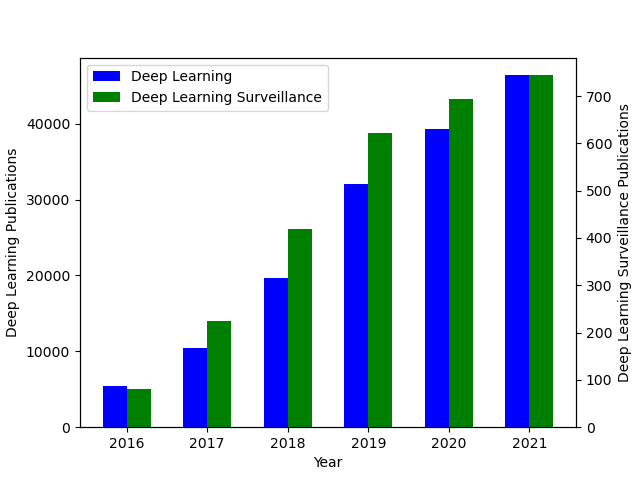
\includegraphics[width=\linewidth]{resources/introduction/publications_graph.png}
    \caption{The increase in publications mentioning the terms "deep learning" and "deep learning surveillance" \cite{deep_learning_surveillance_stats}}
\end{figure}
Yet despite the major progress within the field of deep learning, there are still many tasks where humans outperform models, especially in anomaly detection where the anomalies are often undefined. Deep learning approaches also perform poorly when dealing with noise and concept drift.
\par
The cause for the discrepancy lies in the difference between how humans and machine learning algorithms represent data and learn. Most machine learning algorithms use a dense representation of the data and apply back-propagation in order to learn. Human learning happens in the neocortex, where evidence points to that the neocortex uses a sparse representation and performs Hebbian-style learning. For the latter, there is a growing field of machine learning dedicated to replicating the inner mechanics of the neocortex, namely  \gls*{htm} theory. This theory outlines its advantages over standard machine learning, such as noise-tolerance and the ability to adapt to changing data.
\par
With the advantages of  \gls*{htm} and the rise of video anomaly detection in mind, a natural question one could pose is whether it is possible to apply  \gls*{htm} for anomaly detection in videos. Combined with a lack of related works, it is this very question that is the motivation behind this thesis.
\section{Problem Statement}
Based on the background and motivation, the problem statement can be boiled down to a simple question: \textbf{Is \gls*{htm} viable for use in video anomaly detection?}\par
This thesis will introduce three different tasks that will help answer the question and also showcase the performance of HTM. These tasks will vary in difficulty, complexity, and will focus on different use cases. This thesis will also cover all required knowledge. To summarize, this thesis will cover three objectives:
\begin{enumerate}
    \item Introduce  \gls*{htm} and give a deep understanding of the inner workings, the strengths, and the weaknesses. While also being friendly to readers with a machine learning background.
    \item Develop and outline a theoretically sound pipeline so that  \gls*{htm} can be applied for anomaly detection in complex videos.
    \item Perform tasks, discuss the results, and lay out potential future work.
\end{enumerate}
\section{Limitations}
HTM is a complex topic not part of the curriculum in most educations, if any at all. It is also based on neurological research, lending terms and concepts from the biological field, which significantly raises the level of entry for people with a machine learning background. This makes learning and understanding \gls*{htm} a process which takes up a sizable chunk out of the total time spent on this thesis. This thesis will therefore be relatively limited in scope.
\par
Additionally, \gls*{htm} for video anomaly detection is a novel topic and is therefore naturally limited on several fronts. One of the main limitations is the lack of labeled anomaly data that suits the nature of HTM, because most datasets are made for use with deep learning approaches. Another problem is the lack of works related to applying \gls*{htm} on video-based problems. Finally, while there are other methods that can be used for video anomaly detection, none of them are based on the same premises as HTM. This means that there is a major lack of methods to use for the purpose of benchmarking and comparison.
\par
Last but not least, the \gls*{htm} theory described in this thesis is not the first generation \cite{htm_zeta1}, which was probabilistic in nature. The \gls*{htm} theory described in this thesis is actually the third generation\cite{htm_gen3, thousandbrains}, which builds upon the second generation\cite{htm_gen2_sp,htm_gen2_tm}. The second generation is often referred to as Cortical Learning Algorithms (CLA), which made the move from probabilistic modelling to Sparse Distributed Representation. The third generation builds upon the second generation by introducing concepts such as sensorimotor inference and The Thousand Brains Theory. The first generation had fundamentally different inner workings, but shared a lot of the terms with the current generation. This has made researching  \gls*{htm} challenging as there are many research papers published that refer to the first generation.
\section{Contributions}
This thesis contributes in multiple ways. Not only does it present a novel way to apply  \gls*{htm} on video-based problems, it also uncovers the reasoning behind the design decisions that were made as well as providing thorough analysis.
\par
This thesis also acts as an organization of  \gls*{htm} related research, supported with visualizations and a simpler language, making it easier for people with a machine learning background to understand. It is also important to mention that not only does this thesis include the main HTM research published, but it also contains little tidbits of community research and ideas which are otherwise hard to come by.
\par
Additionally, during the development of the software used in this thesis, contributions have been made to the  \gls*{htm} community in the form of uncovering and reporting a bug related to the technical implementation of  \gls*{htm} \cite{github_contrib}, as well as new high quality figures and visualizations that may aid people that are new to HTM.
\section{Thesis Outline}
This thesis consists of five chapters, where \autoref{sec:introduction} and \autoref{sec:background} are introductory and contain relevant background information for the understanding of the proceeding chapters. \autoref{sec:grid_htm} and \autoref{sec:experiments} present the own work done during this thesis. \autoref{sec:conclusion} neatly summarizes this thesis and presents areas in which there can be performed further work. More details for each of the chapters, except this one, is presented below.
\par
\subsection*{Chapter 2: Background}
\autoref{sec:background} covers the required knowledge for the proceeding chapters. It is split up into three parts. The first part covers the history of deep learning, and has an increased focus on the parts of deep learning that are especially relevant for this thesis, such as generative models.
\par
The second part covers anomaly detection. More specifically, it covers the definition, challenges, and recent work within anomaly detection. It also discusses smart surveillance, which is a subset of anomaly detection specifically meant for surveillance purposes.
\par
The third and final part covers HTM theory. It starts off by introducing the biological ties of HTM and the pipeline of an HTM model. This is then proceeded by a detailed account of the inner mechanisms of an HTM model and how learning is performed. It then finishes by introducing use-cases, related work on the use of HTM for anomaly detection and how it performs, and introduces similarities between recent developments within HTM theory and recent developments within deep learning.
\subsection*{Chapter 3: Grid HTM}
This chapter introduces Grid HTM, a modified HTM network for the purpose of anomaly detection in videos. Grid HTM is presented gradually as problems have to be solved, as well as use cases that suit the properties of the model. The technicalities are explained with the help of figures and textual analysis. This model is then used in \autoref{sec:experiments} when performing experiments.
\subsection*{Chapter 4: Experiments and Results}
This chapter presents three experiments that aim to explore the capabilities and challenges of HTM and Grid HTM in the context of anomaly detection in videos. The first experiment is a controlled experiment where a computer-generated ball is bouncing with anomalies inserted. The aim of this experiment is to test whether the capabilities of HTM apply for videos, as well as the performance of Grid HTM on the same task.
\par
The second experiment showcases the performance of Grid HTM on a surveillance video with technical anomalies. Additionally, several key points of interests and the respective outputs of Grid HTM are shown in order to get a better understanding of its capabilities.
\par
The third experiment further explores the ability of the Grid HTM to detect segments in videos, which was discovered in the previous experiment. The videos that are used in this experiment are videos of sperm that contain several segments.
\subsection*{Chapter 5: Conclusion and Further Work}
In this chapter the thesis is summarized, and the thesis question presented in \autoref{sec:introduction} is answered along with potential further work.